%!TEX root = ../main.tex\
\chapter{Introduction}\label{intro}
\section{What is Reverse Engineering?}

Reverse engineering is the process of disassembling, deconstructing, or analyzing a system, device, or piece of software in order to gain a deep understanding of how it functions. This concept has existed long before its modern applications in technology. For example, the dissections many of us performed in high school biology classes were, in essence, an early form of reverse engineering. Those dissections were carried out to break down something as complex and mystifying as life into understandable components and functions, revealing how various biological systems worked together. Similarly, one of the most effective ways to fully comprehend how a technological system operates is to open it up and inspect it piece by piece.

Reverse engineering software can be accomplished through a variety of techniques. Broadly speaking, these methods fall into two categories: static analysis and dynamic analysis. Static analysis involves studying a snapshot of the code in a single, unchanging state without executing it. This provides insight into how the software is structured, its logic, and potential areas of interest. In contrast, dynamic analysis takes place while the program is actively running, allowing an analyst to observe how it behaves in real time, including how it handles data and responds to inputs. Typically, a reverse engineering process might begin by passing a program’s executable to a disassembler, which translates machine code into assembly-level instructions. From there, a programmer might use system monitoring tools to gather information provided by the operating system about how the program interacts with its environment. Additionally, debuggers allow reversers to observe the CPU’s internal operations, stepping through the disassembled code one instruction at a time to scrutinize the logic behind each operation. Using these various tools, a programmer must rely heavily on intuition, experience, and problem-solving skills to navigate the complex and often opaque process of reverse engineering.

There are numerous reasons someone might choose to reverse engineer software. The only time the inner workings of software are openly accessible to anyone is when it is released as open source. Open source software consists of freely available source code that anyone can read, modify, or distribute. However, developers frequently choose not to make their source code public for a range of reasons, including legal and licensing restrictions, protection of proprietary technologies, or personal business strategies. The opacity of proprietary software often leaves users, researchers, or competing developers with no choice but to reverse engineer if they wish to understand or interact with it.

Some of the most common motivations for reverse engineering software include performing malware analysis, improving one’s programming skills, recovering lost source code, and enabling interoperability between different systems or applications. My own first introduction to the world of reverse engineering came through a video in which the creator was reverse engineering Apple’s FaceTime for Mac. His goal was to reinstate closed captioning functionality for his hearing-impaired mother—a striking example of how reverse engineering can serve highly personal and practical purposes. The potential applications of reverse engineering are as diverse and far-reaching as the software programs that exist today.

Most software developers are familiar with reverse engineering primarily through its use in malware analysis. A classic example of malware is a Trojan virus, in which malicious developers conceal harmful code inside programs that appear harmless. Reverse engineering such programs allows security researchers to break them apart and reveal the hidden malware lurking within. Additionally, modern software development often involves the use of external libraries. In large projects, keeping track of all dependencies and the interactions between different modules can be a formidable challenge. Hackers can exploit this complexity by hiding malicious entry points in these libraries to gain unauthorized access to sensitive information. In many cases, reverse engineering remains the only foolproof method for uncovering the true operations of a program and exposing any hidden threats or vulnerabilities embedded deep within the code.

Another compelling reason to reverse engineer software is to enhance one’s own technical skills. The process requires extensive knowledge of both low-level assembly language and high-level programming concepts. Reverse engineering someone else’s code is no simple feat. It forces the reverser to learn deeply about various methods of structuring and implementing software, as well as the diverse strategies developers use to solve problems. Through this process, reverse engineers often become far more proficient programmers, gaining insight into advanced coding techniques and architectural design choices that might not be visible in standard learning materials. This project itself will serve as an endeavor in learning not only forward engineering but also the intricate art and science of reverse engineering.

Another reason people may reverse engineer software is to recover lost source code. Though this is far from easy, it is sometimes possible to reconstruct high-level source code from compiled executables. Many developers have experienced the frustration and panic that comes with losing source code due to accidental deletion, hardware failures, or lack of proper backups. In such scenarios, reverse engineering can offer a potential solution, providing a lifeline to recover critical work that might otherwise be lost forever.

Interoperability represents yet another crucial motivation for reverse engineering. In many cases, achieving compatibility between different programs, systems, or devices is impossible without reverse engineering. When working with external libraries or operating systems that provide documentation without accompanying source code, developers frequently encounter undocumented behaviors or missing details. While a programmer could attempt to resolve these issues through trial and error or by contacting the vendor, reverse engineering provides a definitive and often faster way to understand how to integrate different systems effectively. It serves as a bridge between incompatible software components, enabling seamless communication and cooperation in ways that might otherwise remain impossible.

\section{Reverse Engineering Methods and Tools}

Because reverse engineering serves a wide variety of purposes, there is an equally broad range of methods and strategies employed to achieve those goals. In \textit{Reversing: Secrets of Reverse Engineering}, these methods are generally categorized into two primary types. The first type focuses on large-scale observation of a program and is referred to as system-level reversing. System-level reversing seeks to determine the overarching structure of a program and identify potential areas of interest within it. Once a general understanding of the program’s layout has been established, the analysis can proceed to the second type: code-level reversing. Code-level reversing delves deeper into the specifics of a program’s inner workings, offering detailed insights into particular segments of code and uncovering how algorithms and functionalities are implemented.

System-level reversing is achieved by running an array of specialized tools on a program and observing the services provided by the operating system. These observations gather information on how the program interacts with system resources, tracks input and output operations, and reveals characteristics of the program’s executable files. Much of this data is supplied by the operating system, as any portion of a program that interacts with components outside itself must necessarily communicate through the OS. As a result, effective system-level reversing demands a strong familiarity with the operating system’s internal workings, making it invaluable for reverse engineers to develop deep expertise in the OS environment they are targeting.

Code-level reversing, by contrast, is a far more complex and meticulous process. It involves extracting algorithms, logic, and design concepts directly from a program’s binary code. This task requires a robust background in reverse engineering techniques, software development practices, CPU architecture, and operating system internals. Even when working with readable, well-documented source code, modern software systems can be enormously complex. For instance, the program examined in this project comprises 21 frameworks, contributions from at least three separate companies, and potentially tens or even hundreds of thousands of lines of code. Moreover, when high-level code is compiled into binary instructions, a single line of code can transform into ten or more lines of low-level machine instructions. Reversing production-level software from binary back to source code is thus an almost incomprehensibly difficult endeavor. Thankfully, multiple methodologies and a variety of specialized tools have been developed to aid in effective code-level reversing, making this seemingly impossible task more approachable for skilled practitioners.

\subsection{Static Analysis}

Static analysis is the practice of analyzing code without executing it. This approach allows reverse engineers to study the structural and logical components of a program in a controlled environment, free from the risks associated with running potentially malicious code. Static analysis can also serve as a valuable precursor to dynamic analysis, helping to identify key areas of interest for more in-depth examination later.

Static analysis tools operate at both the source code level, when code has not yet been compiled, and at the machine language level, analyzing binary or assembly-level code. Reverse engineers frequently use static analysis tools to disassemble machine code into assembly instructions, enabling them to examine and interpret how different sections of code relate to one another. While retrieving disassembled code is one of the most fundamental functions of static analysis tools, many modern tools offer a host of additional features, such as graphical representations of control flow, cross-referencing functions, and identifying potential vulnerabilities. These tools are often designed to provide reverse engineers with a starting point, helping them navigate the often bewildering world of assembly-level functions and binary logic.

\subsubsection{Disassembler}
One of the most key static analysis tools for a reverse engineer is a disassembler. 
Disassemblers are applications that take in a program’s executable file and generate a file with the assembly code.
This isn’t too difficult because assembly is just a text translation of the machine readable binary code. 
Unfortunately, that makes it a lot less clear than higher level programming languages.  
Disassembly is also unique to a person’s processor, but there are disassemblers that can support more than one CPU architecture.
Some examples of disassemblers are IDA, Binary Ninja, Hopper, Ollydbug, Radare2, and Ghidra.

\subsubsection{Decompiler}
Decompilers are similar but more complex than disassemblers.
Instead of just producing the assembly language code, decompilers attempt to produce high-level readable code. 
They attempt to produce something that looks as close to the source code as possible by reversing the compilation process~\cite{Reversing}.
The front end of the decompiler decodes low-level assembly instructions and translates it into an intermediate representation specific to the decompiler. 
The intermediate representation is then iterated on to remove as many extraneous details as possible while preserving the important details. 
Lastly the back end takes the polished up intermediate representation and translates it again into a high level language.

While this may sound like a simple way to retrieve the source code, it is highly unlikely the high level language returned will be something that actually matches. 
Anyone who has ever run text through a translation website multiple times knows that each iteration causes a loss in fidelity and oftentimes the end result will be gibberish. 
Decompilers go a step further and have no immediate knowledge of things like function or variable names and structures. 
This does not make them useless, though. For example, a text translator will usually return your original result when given a simple phrase. 
Similarly a decompiler will most likely be able to pick up on more straightforward functions such as adding a + b. 
Decompilers offer hints and snippets into what the source code may look like which is valuable information for a reverse engineer. 
Most of the examples for disassemblers listed also count as decompilers.

\subsubsection{Dumping Tools}
Executable dumping is usually the first step in reverse engineering a program. 
Executable dumping helps inform a reverse engineer what a program does, how it interacts with external elements, and general knowledge of how a file is structured. 
Using dumping tools, a reverse engineer will start by figuring out what type of file they’re dealing with. 
They will then start to unpack the format. 
Extracting strings will immediately offer insight into what language the source code is written in, what library modules it uses, what kinds of data it is dealing with, and what the goals of program functions may be. 
Other useful information we can retrieve is the layout of the file in memory and what the general logical structure of the file is. Once we know the type of file we also know which tools we can use. 
For example, some debuggers only work with certain high and low level languages. 
Some popular executable dumping programs are ones already built into your machine like DUMPBIN for windows or otool for mac. 

Otool is identifies a file's mach header. 
On systems with a Mach kernel like macOS and iOS, the executable binaries they use will have a mach header. 
All headers have a magic number to identify them. Thin binaries only have that number while fat binaries with fat headers will have locations of the other executable's headers in them.

\subsection{Dynamic Analysis}

Dynamic analysis occurs when a program—or specific sections of it—is executed during the analysis process. This approach provides unique insights into how software behaves in real time, revealing execution paths, input/output relationships, and interactions with external systems. Because running an unknown program can produce unpredictable and potentially harmful results, it is safest to conduct dynamic analysis within a secure, isolated, or sandboxed environment. Virtual machines are commonly used for this purpose, as they are easy to set up, control, and reset between tests.

A wide variety of tools contribute to dynamic analysis. Any tool that executes code and monitors its behavior falls under this category. Some dynamic analysis tools run entire programs to observe overall functionality, while others focus on specific sections, functions, or even single instructions. Additionally, tools that monitor a program’s external environment during execution—for example, capturing network traffic, tracking file system changes, or observing registry modifications—are also considered part of dynamic analysis. Together, these tools give reverse engineers a powerful way to understand not just how a program is built, but how it behaves in practice.

\subsubsection{Debugger}
Debuggers are a tool usually used for developers to locate and work through errors in their programs, but they’re also vital tools in reverse engineering. 
Many debuggers can work through assembly language. 
While assembly language may be difficult for a human to parse through, it is the exact same logic that gets broken down and sent to a computer meaning that the computer can show what each assembly instruction is intended to do. 
Most debuggers software engineers use were actually designed from the ground up with the purpose of stepping through assembly code. 
The debugger can show the state of CPU registers along with a memory dump that shows what’s in the stack. 
Debuggers usually contain disassemblers which as discussed is a vital reverse engineering tool. 
Many debuggers also contain both software and hardware breakpoints. 
Software breakpoints are instructions added into the code during runtime to pause and hand control over to the debugger. 
Hardware breakpoints are a CPU feature which allow the processor to pause execution when a certain memory address is reached and hand control over to the debugger. 
A reverse engineer can use insert breakpoints at data structures of interest and use the debugger to reveal what they are. 
Debuggers also offer a clear view of registers and memory to aid in a reverse engineer's ability to process low level information.

\paragraph{\underline{User Mode Debuggers}}
Most debuggers that a programmer will use are user mode debuggers.
They run on a system like any other application then seize control of the target program to debug ~\cite{Reversing}.
An advantage to them is that they are easier to set up and navigate than their kernel-mode counterparts.
Usually it’s fine to stay limited to user mode viewing of an application. 
It only creates troublesome limitations when the target application has kernel mode components such as device drivers. 
User mode debuggers are also not always sufficient when trying to debug a program before it reaches the main entry point. 
These kinds of programs are usually ones that have a lot of statically linked libraries in the executable. 
The final and most likely to be problematic issue is that user-mode debuggers can only view a single process in a program. 
This can cause issues when the target application has processes that interact in unknown ways. 
The user may not know which process to zero in on that has the code of interest.

\paragraph{\underline{Kernel Mode Debuggers}}
Kernel mode debuggers are different from user-mode debuggers because they capture the entire system and not just a single process. 
Instead of running atop the operating system, kernel mode debuggers sit alongside the system kernel and stay ready to capture the entire system’s stats. 
Kernel mode debuggers can be more helpful to reverse engineers because they offer more clues as to what’s going on with the system. 
A key tool for kernel-mode debuggers is that they allow the placement of low level code breakpoints. 
As a reverse engineer working with assembly code, being able to test different sets of assembly instructions that may be the code section a reverser is looking for is incredibly useful.

For example, picture a scenario where a reverse engineer is looking for the API responsible for handling moving windows? 
That will need to be managed by a windows manager in the kernel. 
The complexity is introduced when trying to identify which API moves a particular window. 
Since there are multiple APIs that can be used to move a window, pinpointing the one you are trying to focus on is a difficult task. 
This is where kernel mode debuggers come in handy. 
Low level breakpoints in the operating system responsible for shifting windows around will help you identify which API is getting called when a window is moved~\cite{Reversing}. 
From there the reverse engineer will be able to hone in on that API.

Unfortunately, kernel mode debuggers come with their own drawbacks. 
Setting them up can be challenging because they require access to the full system. 
They need to suspend the entire system while running so they can go line by line, which means the system can no longer have multiple threads going~\cite{Reversing}. 
They will also usually need to be set up inside a Virtual Machine which will be discussed in a later section~\cite{PracticalRE}. 
These are reasons why a reverser should exhaust their other options before jumping into using a kernel mode debugger. 
Still, they are powerful tools when the scenario calls for it.

\subsubsection{System Monitor}
System monitoring can be a crucial part of the reverse engineering process. 
In some cases, a reverse engineer can figure out what they need through system monitoring tools without ever looking at the decompiled code. 
System monitoring tools can capture what happens between the code and hardware using the intermediate channels of input/output~\cite{Reversing}. 
For local system monitoring, tools monitor things such as file operations (creating, deleting, moving, etc). 
For programs that communicate over networks, system monitoring might look like recording all TCP/UDP network traffic. 
System monitoring tools are commonly used in virtual machines.


\subsubsection{Virtual Machine}
Many programmers will encounter virtual machines (VM) at some point during their career. 
It’s not uncommon for an application to interface exclusively with one type of operating system. 
One reason is because writing applications to work with different operating systems adds time and complexity that not all programmers can afford.
Choosing to write in a high level language may make code more portable because there’s more verbose built-in libraries or interpreters that deal with the specifics of the systems without the need for any programmer intervention.
But high level languages often trade performance for convenience which is not a trade that a developer working with large amounts of data can necessarily afford to take.
What happens when a developer has an application that runs on Windows while they have a Mac? 
This is where a virtual machine enters into the mix. Virtual machines are safe sandboxed environments that work as miniature computers with their own operating systems within a computer. 
They are constructed with an interpreter and bytecode. 
During compile time, select code snippets are compiled specific for the VM target architecture and then inserted into the program along with the interpreter. 
During run-time, the interpreter begins executing the bytecode. 
Virtual machines are costly to implement because they are so expansive which is why only the necessary code snippets get rendered~\cite{MasteringRE}.
Because virtual machines work in their own isolated environment, they offer powerful protections against unknown or potentially malicious software. 
This makes them a useful tool for reverse engineers who deal with software that they do not know the contents of. 
The level of control over virtual machines also makes them a useful tool because there is ultimate knowledge of system conditions.


\section{Protocol Analysis}

Communication protocols form the essential foundation for structured exchanges of information between different systems and components. Many applications, especially those that involve interoperability between different platforms or devices, depend on well-defined formats for sending and receiving messages. However, in cases where official protocol specifications are unavailable, incomplete, or proprietary, protocol reverse engineering can be a crucial tool for discovering the format, flow, and logic behind these communications.

Protocols are extensively used in telecommunications, networking, and distributed systems because they establish consistent rules for exchanging data between different entities. Protocols may be published as open standards, freely accessible for anyone to implement, or they might be kept proprietary, obscuring their details from end users and competitors. Protocol reverse engineering is most often employed in the latter scenario, where understanding the communication mechanisms is critical but official documentation is unavailable. The primary objective of protocol reverse engineering is to derive a model of how the target protocol functions, without any prior knowledge of its inner workings.

Protocol reverse engineering also plays a vital role in simulating network protocols. Network simulation allows researchers and developers to rapidly prototype specific test cases that might be cumbersome, time-consuming, or even impossible to execute in real-world environments. Furthermore, simulation tools can replay captured network traces under different conditions, helping engineers adapt their systems to new requirements or environments. In cybersecurity, protocol reverse engineering is frequently used in software security audits to verify that components behave correctly and securely under a range of circumstances, identifying potential vulnerabilities or compliance issues before they can be exploited.

Another significant application of protocol reverse engineering is network conformance testing, where the protocol in question is already known. In these cases, reverse engineering can help create a detailed model of the protocol’s behavior, which can then be compared to official standards or specifications to ensure that an implementation adheres to the expected rules and practices.

There are two general categories of protocol reverse engineering techniques. The first focuses on analyzing the messages exchanged between two components on a network. By carefully examining these exchanges—often referred to as network traces—analysts can infer the structure, commands, and responses that define the protocol’s behavior. The second approach involves reverse engineering the application itself. This can mean analyzing the source code (when available), disassembling binary code, or tracing sequences of binary instructions during execution to reveal how the protocol logic is implemented internally~\cite{stateofartRE}.

Many tools exist to automate significant parts of the protocol reverse engineering process. The initial setup phase typically involves identifying and characterizing the operating environment in which the protocol operates. With a solid understanding of the environment, analysts can begin the observation phase, which involves using specialized tools to collect network traffic or execution traces. Once data has been gathered, it must be sanitized to extract only the relevant messages associated with the target protocol, filtering out noise and unrelated data. The final step is the actual analysis, where analysts draw inferences about the protocol’s structure, message formats, and state machines. These steps are highly iterative and rely heavily on the expertise and insight of the analysts, as well as the capabilities of the tools being employed. Figure~(insert number) illustrates this step-by-step process.

\begin{figure}[h]
	\caption{Piconet Topology}
	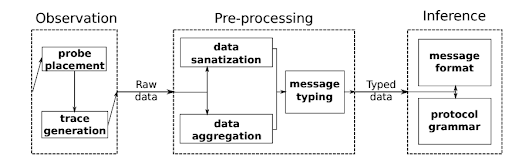
\includegraphics{protocol_analysis_process.png}
\end{figure}

